\section{Motivation}
\label{chap:Motivation}


The economy and the welfare of humanity depend on a functional healthcare system. There has been a significant amount of change between the world we live 
in today and the one we did a few decades ago. Everything has become more disorganized and ugly. In this case,
 medical professionals are risking their own lives in order to save as many lives as they possibly can.

 Board-certified medical professionals known as virtual doctors prefer to do phone and video consultations over in-person 
 consultations when they can, however this is not always possible in an emergency. Machines are considered to be 
 superior to humans in the absence of human error because they can do tasks more quickly while keeping a constant 
 degree of precision. Without involving a person, a disease predictor, also referred to as a virtual doctor, can 
 correctly forecast a patient's illness. In severe cases, like COVID-19 and EBOLA, a disease predictor can save a 
 person's life by identifying their health without the need for physical contact. There are virtual doctors 
 available now, but they lack the ability to offer the necessary level of precision.

Doctors may make mistakes when diagnosing a patient's disease, but disease prediction systems with machine learning 
algorithms can help produce accurate results in these situations. For this project, we employed a mix of approaches
, algorithms, and technologies to develop a system that can forecast a patient's status based on hospital data and
 machine learning methods based on the Python programming language. 
 Following that, the data is categorized using the K-NN algorithm.
\\

\section{Approach}
\label{chap:Approach}
\subsection{Dataset}
\label{sec:Dataset}

This inquiry used data from Kaggle.It's A dataset to provide the students a source to create a healthcare related system
There are columns containing diseases, their symptoms , precautions to be taken, and their weights.
This dataset can be easily cleaned by using file handling in any language. The user only needs to understand how rows and coloumns are arranged.
\newpage
\begin{figure}[htp]
    \centering
    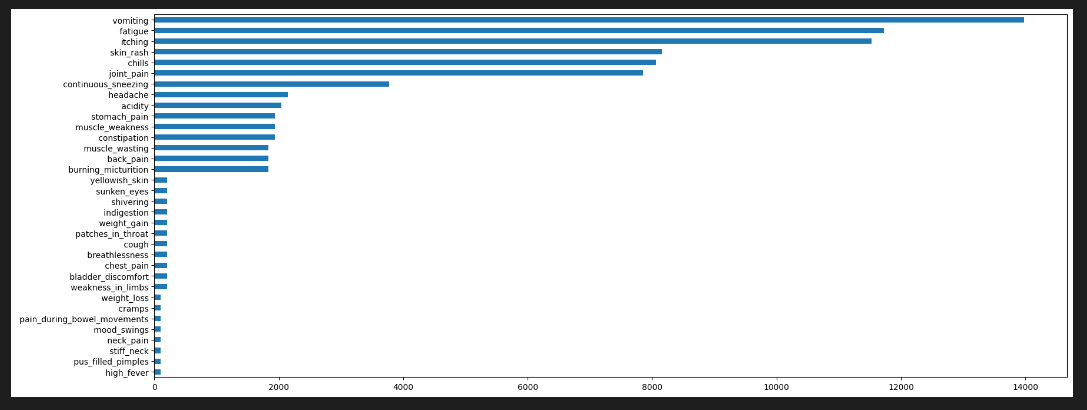
\includegraphics[width=0.9\textwidth]{images/dataset.png}
    \caption{Image of desease distribution in the dataset}
    \label{fig:example1}
\end{figure}

\subsection{ Proposed System}
\label{sec:Proposed System}
In the suggested strategy, we use Machine Learning techniques and a web interfaceto precisely forecast the ailment that the patient has been suffering from.
 When past healthcare records are used as a dataset, the results are more accurate. 
 To train the model and predict user diseases based on the symptoms they enter, 
 we use machine learning algorithms.\\
\textcolor{red}{\underline{\textbf{Advantages of Proposed System\\}}
}
 \begin{itemize}
    \item\textbf{First and foremost, seeing a doctor for modest treatment is unnecessary.} 
    \item\textbf{When compared to past treatments, you'll get more precise results} 
    \item\textbf{Only a few risk variables are at play} 

\end{itemize}

\section{Model and algorithm}
\label{chap:apprModel and algorithmoach}
To construct a disease prediction based on symptoms, we applied 2 machine learning algorithms: 
 Random Forest, KNN. We can get an accurate forecast for our model using
 these tactics. The Prognosis of the Illness Currently, the effort is in full swing. Machine Learning is
  being used to diagnose and prevent disease in its infancy. As we all know, humanity has become so engrossed 
  in the competitive environment of economic advancement that it has lost sight of its own well-being. Studies
   show that 40 percent of people ignore small symptoms, which might lead to more serious problems in the future. 
   The project's interface is also built with Flutter. The user must first enter their
    name, then select symptoms cases; alternatively, the user must enter all symptoms, after which 
    the system will return an exact result. Two machine learning approaches were used to create this forecast:
   Random Forest, KNN. When the user enters all of the symptoms and simply 
     presses the Predict Button, the result is computed ; similarly, we've utilized four
      ways to provide a more thorough perspective of the data, and the user must be satisfied with the anticipated 
      conclusion.

\subsection{Activation function}
\label{sec:Activation function}
  \todo[inline]{\Large\textbf{ Random Forest}}
  Random Forest, a well-known machine learning algorithm, employs the supervised learning method. In machine learning, 
  it can be utilized for both classification and regression issues. It is based on ensemble learning, which is a method for
   solving a complicated problem by merging numerous classifiers and improving the model's performance.
    \begin{figure}[htp]
        \centering
        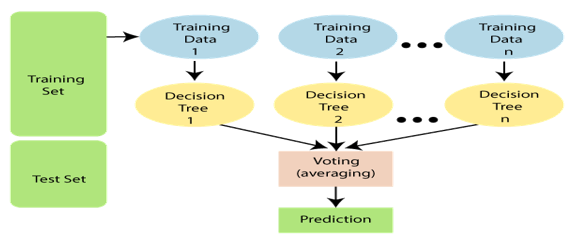
\includegraphics[width=0.7\textwidth]{images/randomforest.png }
        \caption{sigmoid and ReLu }
        \label{fig:example4}
    \end{figure}
  
    \todo[inline]{\Large\textbf{ KNN}}
    One of the most fundamental Machine Learning algorithms is the K-Nearest Neighbour approach. It is based on the method of
     Supervised Learning. Because K-NN considers the new case/data and previous cases to be comparable, the new case is assigned to the category that is the most similar to the previous categories.
\\
The K-NN method keeps track of all available data and categorizes new data points based on how similar they are to existing data. As fresh data arrives,
 the K-NN algorithm can quickly filter it into the appropriate suite category. Although this method can be used for both regression and Classification, classification is the most popular use.

    \begin{figure}[htp]
        \centering
        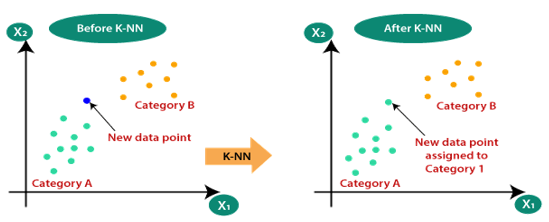
\includegraphics[width=0.9\textwidth]{images/KNN.png }
        \caption{Neural Network }
        \label{fig:example4}
    \end{figure}

\section{Experiment and Results}
\label{chap:Experiment and Results}

\subsection{Experimentation}
\label{sec:Experimentation}

To conduct all of the experiments in 
the Jupyter notebook, we used the python3 programming language on one hand and for testing purpose we used Azur Machine learning with an embedded  python script
 to deploy a webservice Later
\begin{figure}[htp]
    \centering
    \includegraphics[width=0.9\textwidth]{images/azure.png}
    \caption{Azure Machine learning }
    \label{fig:example4}
\end{figure}

\begin{figure}[htp]
    \centering
    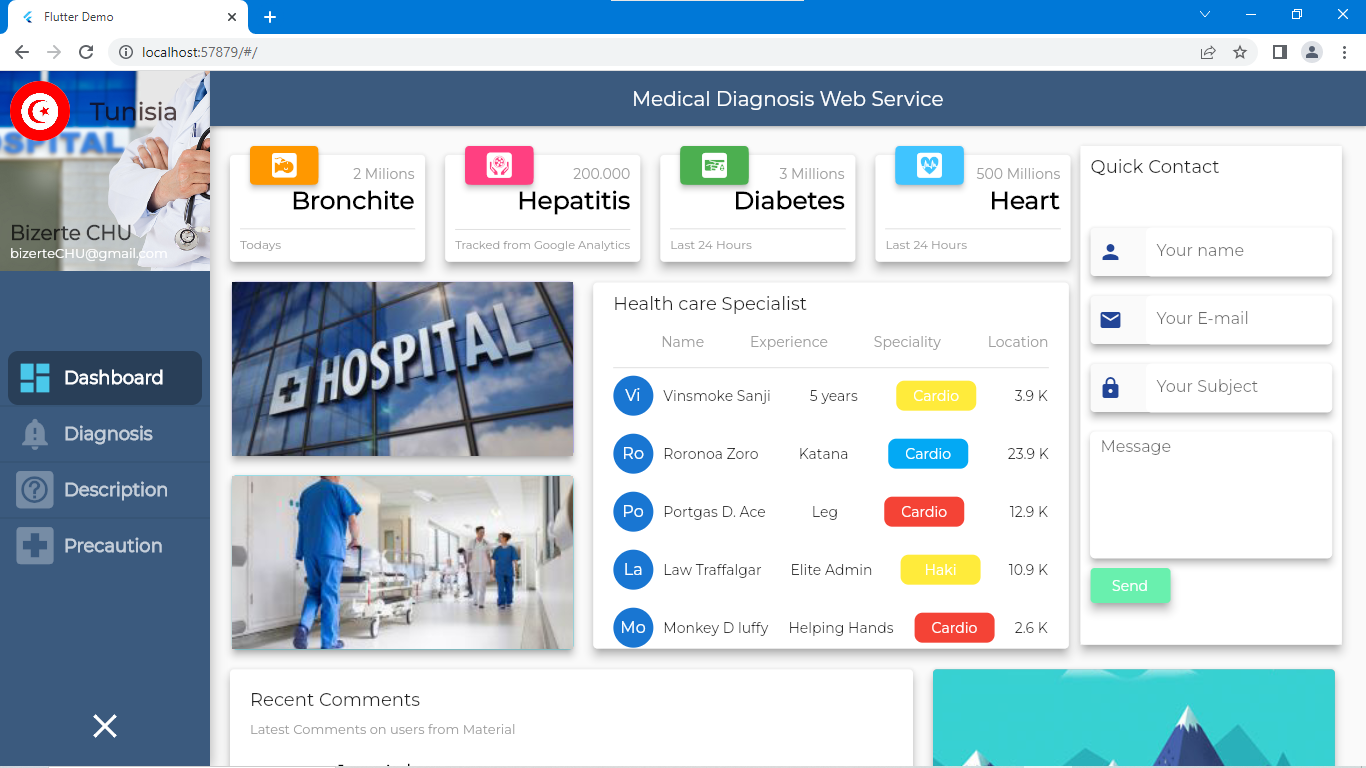
\includegraphics[width=0.9\textwidth]{images/web.png}
    \caption{Web interaface build with Flutter }
    \label{fig:example4}
\end{figure}

\subsection{Metrics for Assessment}
\label{sec:Metrics for Assessment}

\todo[inline]{\Large\textbf{ Metrics for Assessment}}
We get accurate disease prediction because we supply symptoms as input to the system
\begin{figure}[htp]
    \centering
    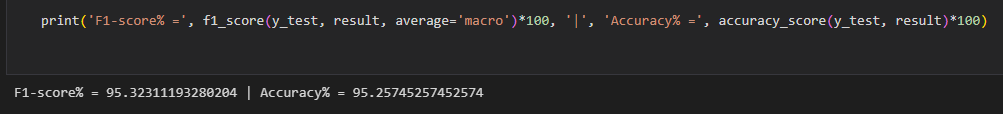
\includegraphics[width=0.6\textwidth]{images/metric.png}
    \caption{Confusion Matrix }
    \label{fig:example5}
\end{figure}

 \subsection{Disease Prediction Dataset}
 \label{sec:Disease Prediction Dataset}
\todo[inline]{\Large\textbf{Disease Prediction Dataset}}

A CSV data file from New York-Presbyterian Hospital was provided by the University 
of Columbia. The Deseases Symptoms data file has 4920 rows and 18 columns while the deseases severity have 133 rows and 2 columns.
Itching, skin rash, shivering, chills, joint stiffness, and other symptoms are some of the most prevalent attributes.
After the preprocessing step There is a total of 18 columns in the dataset out of which 17 columns represent the symptoms and the last column is the prognosis.

\begin{figure}[htp]
    \centering
    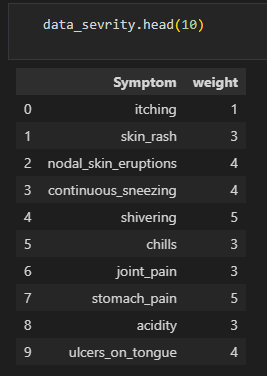
\includegraphics[width=0.3\textwidth]{images/dataseverity.png}
    \caption{Severity Dataset }
    \label{fig:example5}
\end{figure}

\begin{figure}[htp]
    \centering
    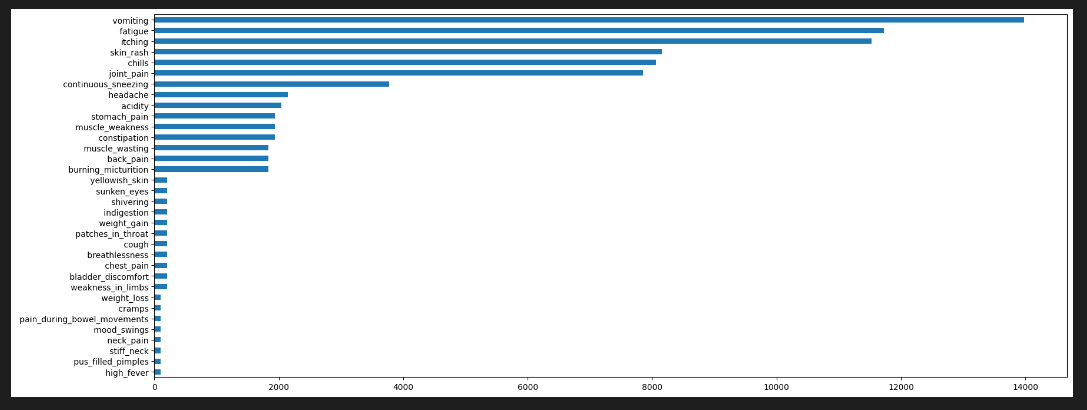
\includegraphics[width=0.7\textwidth]{images/dataset.png}
    \caption{Reaprtition Symptoms in dataset}
    \label{fig:example5}
\end{figure}


\subsection{Data Preprocessing}
\label{sec:Data Preprocessing}

This step will remove any punctuation,delete null,replace symptoms by their weigth
\begin{figure}[htp]
    \centering
    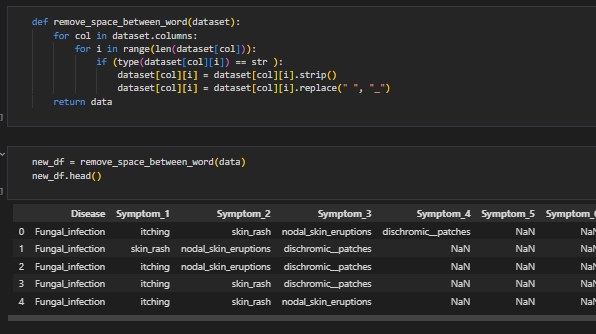
\includegraphics[width=0.9\textwidth]{images/preprocessing.png}
    \caption{Preprocessing}
    \label{fig:example}
\end{figure}


\subsection{Training/Results}
\label{sec:Training/Results}
The system will compare the user's symptoms to the dataset as they are entered, the dataset is made up of binary 0s and 1s, and once the model 
has assessed all of the user's symptoms, it will accurately forecast the disease associated with that manifestation.

\begin{figure}[htp]
    \centering
    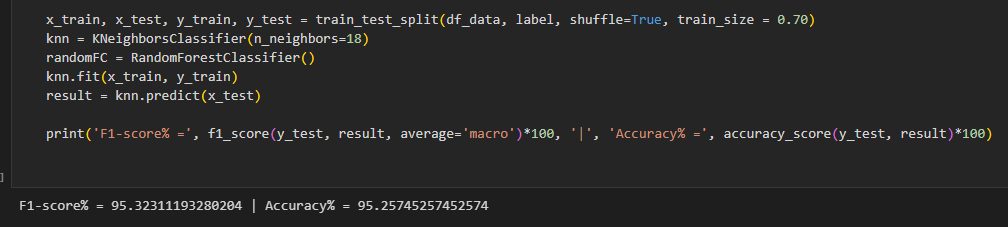
\includegraphics[width=1.2\textwidth]{images/Traning.png}
    \caption{Training Results}
    \label{fig:example}
\end{figure}



\subsection{Prediction/ Outputs}
\label{sec:Prediction/ Outputs}
The system will compare the user's symptoms to the dataset as they are entered, the dataset is made up of binary 0s and 1s, and once the model 
has assessed all of the user's symptoms, it will accurately forecast the disease associated with that manifestation.

\begin{figure}[htp]
    \centering
    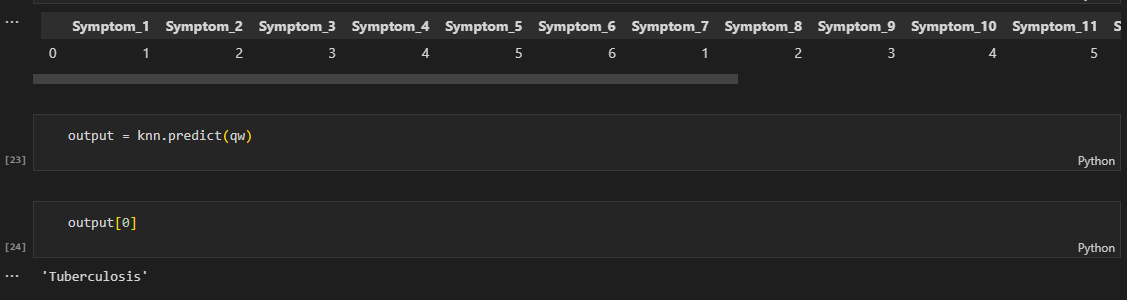
\includegraphics[width=1.2\textwidth]{images/prediction.png}
    \caption{Exemple of Prediction}
    \label{fig:example}
\end{figure}

\begin{figure}[htp]
    \centering
    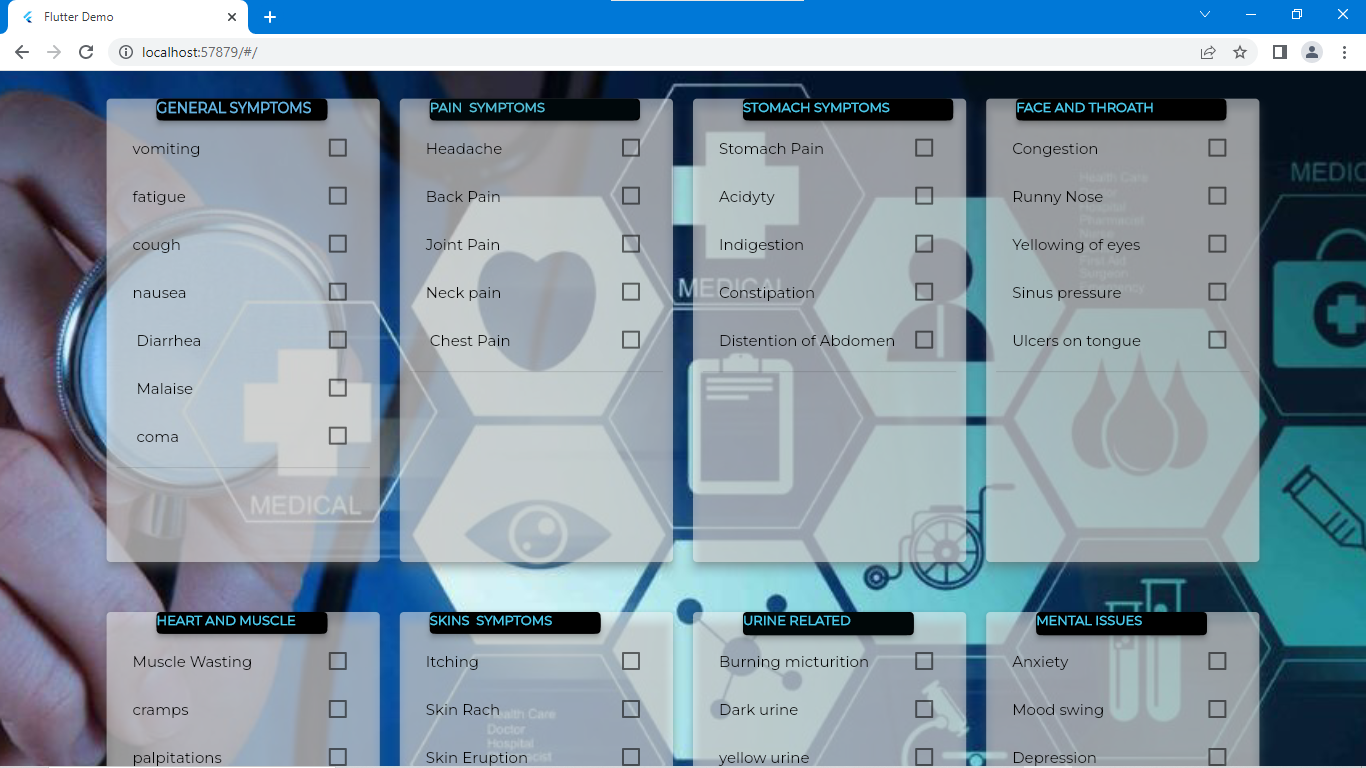
\includegraphics[width=0.9\textwidth]{images/Web1.png}
    \caption{Web interface diagnosis page}
    \label{fig:example9}
\end{figure}

\newpage

\section{Conclusion}
\label{chap:conclusion}
Last but not least, I'd like to stress how crucial this project—disease prediction using machine learning—is 
to everyone's daily lives, but especially to those in the healthcare sector, who use these systems frequently to forecast patients' diseases based on their general characteristics and symptoms. 
Since the health sector now plays such a significant role in treating patients' illnesses, it is frequently quite beneficial for the sector to inform the user. It is also helpful for the user if
 he or she does not want to visit a hospital or other clinics because the user can learn about the disease they are experiencing by simply entering the symptoms and any other pertinent information, and the sector can 
 also profit from this system. If the healthcare sector adopts this idea, doctors' workloads will be reduced and they will be better able to predict a patient's illness.


\todo[inline]{
A method known as disease prediction allows doctors to anticipate the development of a variety of common diseases that, if untreated or ignored, can cause death and a host of other issues for the patient and their family.
}
\newpage